\documentclass[twocolumn]{revtex4}

\usepackage{graphicx,amsmath}

\newcommand{\bra}[1]{\left< #1 \right|}
\newcommand{\ket}[1]{\left| #1 \right>}
\newcommand{\braket}[2]{\left< #1 | #2 \right>}
\newcommand{\innerp}[3]{\left< #1 | #2 | #3 \right>}

\newcommand{\picwidth}{0.66\linewidth}

\begin{document}

\title{Artificial Atoms: Modeling the Inductively-Shunted Cooper Pair
  Box}
\author{John O'Connor, Jens Koch, Steven Girvin, Vlad Manucharyan, Lev
  Bishop, Schoelkopf et al, Devoret et al}

\date{\today}

\begin{abstract}
  The Cooper pair box is a well-studied quantum circuit that can be
  function as an artificial atom. The inductively-shunted Cooper pair
  box (CPBL) is much less well-studied. Adding an inductive shunt
  promises to mitigate ambient charge noise around the circuit, but it
  also produces a Hamiltonian with completely different
  characteristics. The first examples of these circuits are being
  studied in by Vlad Manucharyan, and while computer models of the
  energy spectrum for these circuits exist, they are too slow to be
  helpful in interpreting the experimental data. We develop a more
  efficient model that is fast enough to run curve fitting on
  experimental data, and demonstrate the results of this model.
\end{abstract}

\maketitle

\section{Introduction}

Quantum computing offers a number of enticing theoretical speedups
over classical computers. Best known is Peter Shor's factoring
algorithm, which can factor large composite numbers in polynomial
time. This has the potential to break popular cryptographic schemes
like RSA that rely on the intractability of the factoring
problem. Another less dramatic but more widely applicable speedup is
Grover's algorithm for searching an arbitrary space of $n$ elements in
time $O(n)$, a quadratic improvement over the classical case. These
and other quantum algorithms have motivated significant research in
the field of quantum computing.

The greatest obstacle to constructing a quantum computer has been to
create the quantum bits (qubits) that store information in
superposition. Any quantum system tends to decohere due to
interactions with its environment, and a qubit has to meet two
contradictory requirements. First, it must be sufficiently decoupled
from its environment to hold its state long enough to perform
meaningful computation. At the same time, though, it has to be coupled
to its environment enough to be reliably measurable with the
computation is finished. This is difficult enough that, at present,
one of the largest quantum computations ever performed
\cite{Vandersypen} was the factorization of the number $15$.

One of the fields in which research is proceeding on this front is
circuit quantum electrodynamics. Quantum circuits have several
potential advantages over other forms of qubits. They sit on a chip
rather than migrating through space, which greatly simplifies research
compared to various atomic methods, and they can be manufactured using
fairly standard circuit printing techniques. More importantly, while
atomic systems have fixed energy spectra, researchers can tune the
parameters of their quantum circuits to produce artificial atoms with
a range of different spectra.

\section{Modeling the Cooper Pair Box}

\begin{figure}
  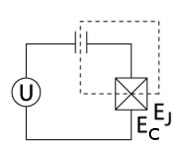
\includegraphics[width=\picwidth]{CPB-circuit.png}
  \caption{A diagram of the Cooper Pair Box. Note that $E_C$ and $E_J$
    are both parameters of the Josephson junction.}
  \label{cpb-circuit}
\end{figure}

One well-studied example of a quantum circuit is the Cooper Pair Box
(CPB). See Fig.\ \ref{cpb-circuit}. We used the basic CPB as an initial
test of our modeling techniques, and we use it here as an introduction
to the inductively-shunted CPB (CPBL). The CPB is a superconducting
circuit with three components: a voltage source, a gate capacitor, and
a Josephson junction.

%
% Consider adding an image of the Josephson junction.
%

A Josephson junction is a circuit element consists of two
superconducting leads joined across a thin insulating boundary. In our
devices, Josephson junctions are constructed by depositing a layer of
aluminum, allowing a thin oxide layer to form on the surface of that
layer, and finally depositing a second layer of aluminum on top. The
oxide acts as an insulator, and at sufficiently low temperatures the
aluminum leads become superconducting. A Josephson junction acts like
a capacitor across its insulating layer, but it also allows Cooper
pairs of electrons to tunnel through. We can treat the Josephson
junction as a capacitor and a tunneling junction in parallel, and we
denote the capacitance and tunneling coefficient of these virtual
components by $E_C$ and $E_J$, respectively.

The capacitative properties of the Josephson junction, together with
the gate capacitor, create a superconducting island in the CPB,
indicated by the dotted line in Fig.\ \ref{cpb-circuit}. This lets us
treat the CPB in its ``charge basis,'' where each eigenstate denotes
a number of Cooper pairs added to or removed from the island. In the
charge basis, the Hamiltonian of the CPB is
\begin{align}
\label{cpb-H}
\begin{split}
  H = \sum_{n=-\infty}^{+\infty}& \frac{-E_J}{2}\left(
      \ket{n}\bra{n-1} + \ket{n-1}\bra{n} \right) \\
    & {} + 4E_C(n-N_g)^2\ket{n}\bra{n},
\end{split}
\end{align}
where $n$ represents the number of tunneled electron pairs and $N_g$
is the offset charge across the capacitor.

In order to calculate the energy spectrum of the CPB as a function of
the offset charge, $N_g$, we will need to express that Hamiltonian as a
matrix in the charge basis. Note that $H$ will be an infinite matrix
not just downward and rightward but, because $n$ and $m$ can take all
integer values, leftward and upward as well. Each matrix element
$H_{nm}$ is equal to the inner product $\innerp{n}{H}{m}$, and so
specifying the matrix only requires specifying those
products. Eqn.\ \ref{cpb-H} gives us:
\begin{equation}
  \innerp{n}{H}{m} = \left\{\begin{array}{lcr}
        4E_C(n-N_g)^2 & : &n=m \\
        \frac{-E_J}{2} & : &|n-m|=1\\
        0 & : & \text{otherwise}
        \end{array}\right.
\end{equation}

Truncating this tridiagonal matrix allows us to approximate its
eigenvalues numerically. The eigenvalues depend only on the ratio
between $E_J$ and $E_C$, and we can plot the energy spectra relative
to $N_g$ for several values of this ratio. We can see that for values
near $0$ where $E_J$ is dominant (Fig.\ \ref{cpb-1}) the spectrum
looks like a series of parabolas, which results from the quadratic
term on the diagonal of $H$. For larger values the spectral lines move apart,
beginning to approximate a constant spacing.

\begin{figure}
  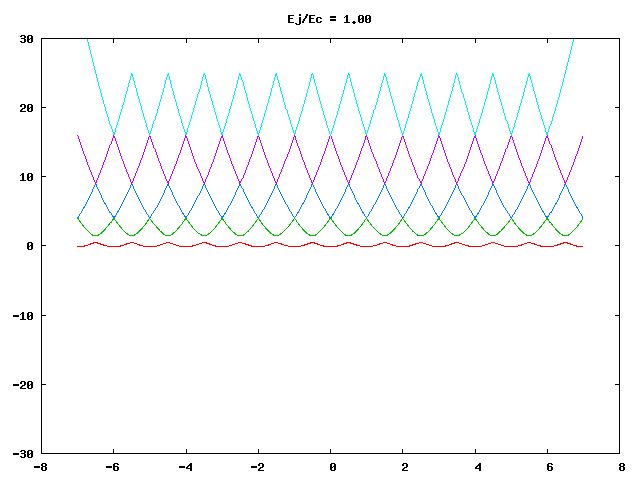
\includegraphics[width=\picwidth]{CPB-1.png}
  \caption{Energy spectrum for the CPB with $\frac{E_J}{E_c}=1$}
  \label{cpb-1}
\end{figure}
\begin{figure}
  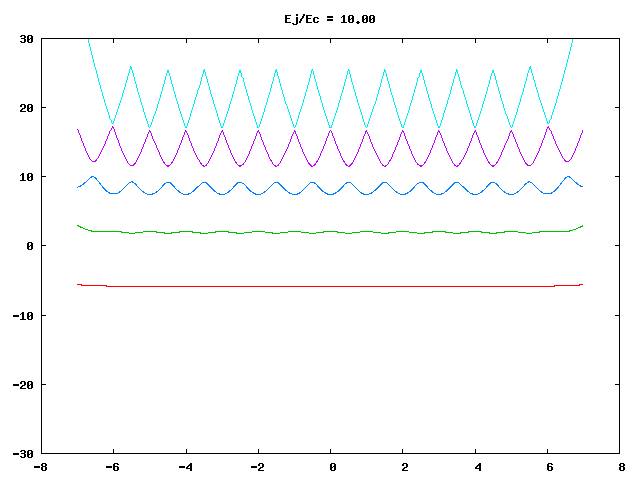
\includegraphics[width=\picwidth]{CPB-10.png}
  \caption{Energy spectrum for the CPB with $\frac{E_J}{E_c}=10$}
  \label{cpb-10}
\end{figure}
\begin{figure}
  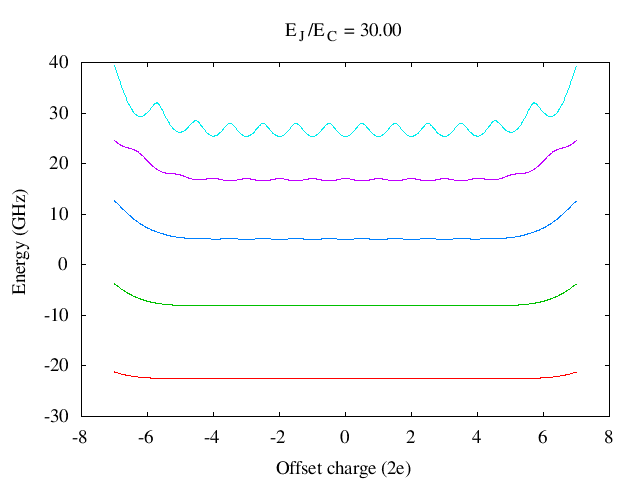
\includegraphics[width=\picwidth]{CPB-30.png}
  \caption{Energy spectrum for the CPB with $\frac{E_J}{E_c}=30$. Note
    that the rising curves on the left and right are an artifact of
    the approximation process, not of the theory itself.}
  \label{cpb-30}
\end{figure}

\section{Challenges with the CPB}
As with all quantum circuits, one of the primary goals is to lengthen
the time before decoherence. In the case of the CPB, one of the
primary causes of decoherence is the charge noise---slow, randomly
oscillating charges in the environment that introduce noise into the
offset charge, $N_g$.

Several strategies exist for mitigating the effects of charge noise in
the CPB. One approach is to operate the device near local extrema of
the energy spectrum. We can see in Fig.\ \ref{cpb-1} that at certain
values of $N_g$ all of the spectral lines of the CPB reach local
maxima or minima. In particular for that figure, the maxima of the
ground level and the minima of the first excited state are both fairly
smooth. When the CPB is operated at these points, the first order
effects of charge noise drop out, though this technique is limited by
the precision of $N_g$.

Another approach is to operate the CPB in the ``transmon'' region
where $EJ\ll EC$. We can see in Fig.\ \ref{cpb-30} that the spectral
lines become very flat, reducing the effects of charge noise even
further. One of the difficulties of working in the transmon region is
that, as we mentioned earlier, the spacing between spectral lines
becomes uniform. This makes the energy differences between states
small integer multiples of one another. Because a qubit generally
needs to be restricted to two energy states, this accessibility of the
higher states can be a substantial problem.

\begin{figure}
  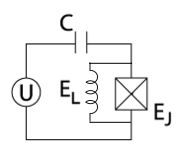
\includegraphics[width=\picwidth]{CPBL-circuit.png}
  \caption{ A diagram of the inductively shunted Cooper pair box
    (CPBL). The circuit now has three parameters, $E_C$ and $E_J$
    associated with the Josephson junction, and $E_L$ associated with
    the inductor.}
  \label{CPBL-circuit}
\end{figure}

A third option---the option that we explore here---is to add an
inductive shunt to the CPB (Fig.\ \ref{CPBL-circuit}).

\section{Modeling the Inductively Shunted Cooper Pair Box}


\begin{thebibliography}{9}
\bibitem{Byrd} R. H. Byrd, P. Lu and J. Nocedal. ``A Limited Memory
  Algorithm for Bound Constrained Optimization.'' \textit{SIAM Journal
    on Scientific and Statistical Computing} 16, 5,
  pp. 1190-1208. (1995)
  
\bibitem{Vandersypen} L. Vandersypen et al. ``Experimental realization
  of Shor's quantum factoring algorithm using nuclear magnetic
  resonance.'' \textit{Nature} 414, pp. 883-887. (20 December 2001)
  
\bibitem{Zhu} C. Zhu, R. H. Byrd and J. Nocedal. ``L-BFGS-B, FORTRAN
  routines for large scale bound constrained optimization.''
  \textit{ACM Transactions on Mathematical Software} Vol 23, Num. 4,
  pp. 550 - 560. (1997)

\end{thebibliography}

\end{document}
